%
%  =======================================================================
%  ····Y88b···d88P················888b·····d888·d8b·······················
%  ·····Y88b·d88P·················8888b···d8888·Y8P·······················
%  ······Y88o88P··················88888b·d88888···························
%  ·······Y888P··8888b···88888b···888Y88888P888·888·88888b·····d88b·······
%  ········888······"88b·888·"88b·888·Y888P·888·888·888·"88b·d88P"88b·····
%  ········888···d888888·888··888·888··Y8P··888·888·888··888·888··888·····
%  ········888··888··888·888··888·888···"···888·888·888··888·Y88b·888·····
%  ········888··"Y888888·888··888·888·······888·888·888··888··"Y88888·····
%  ·······························································888·····
%  ··························································Y8b·d88P·····
%  ···························································"Y88P"······
%  =======================================================================
% 
%  -----------------------------------------------------------------------
% Author       : 焱铭
% Date         : 2023-07-04 21:20:55 +0800
% LastEditTime : 2023-07-05 13:40:59 +0800
% Github       : https://github.com/YanMing-lxb/
% FilePath     : \SCI-LaTeX-Submission-Process-for-Elsevier\2-Manuscript-EN\Section\Section4.tex
% Description  : 
%  -----------------------------------------------------------------------
%


\section{Results and discussion}

\subsection{Numerical validations}
To verify the accuracy of this simulation scheme, the numerical results are compared with the experimental data of several experiments \cite{Zhang.Wu.ea_2022,Qu.Mudawar_2002,Yang.Wang.ea_2017}, as shown in \cref{fig:Verification}.
\begin{figure*}[htbp]
    \centering
    \scriptsize% 设置字体大小
    \subfloat{
        \label{fig:Zhang}
        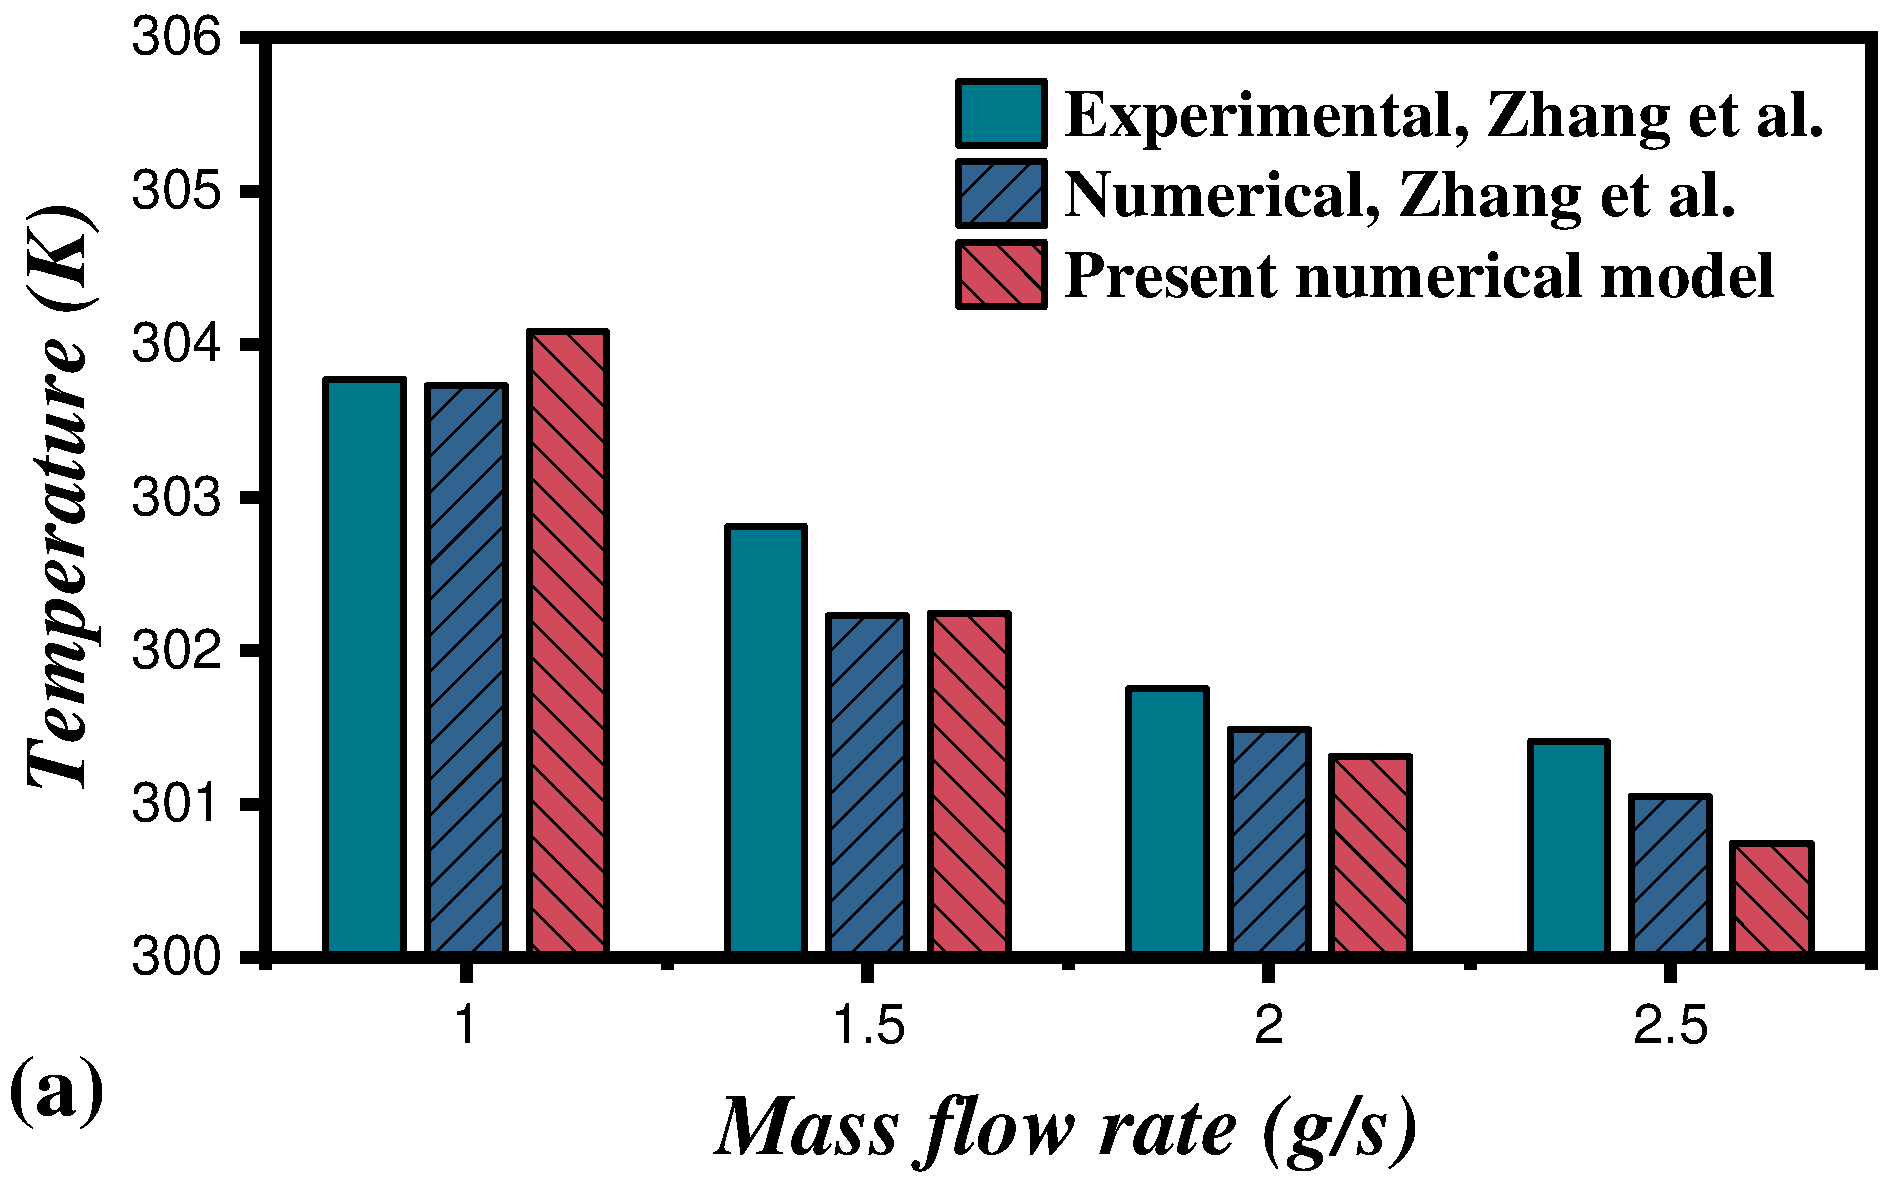
\includegraphics[width=0.35 \textwidth]{V-Zhang-T.pdf}} % 两个\subfloat之间加回车,图片会换行\hspace{2mm}
    \subfloat{
        \label{fig:Qu}
        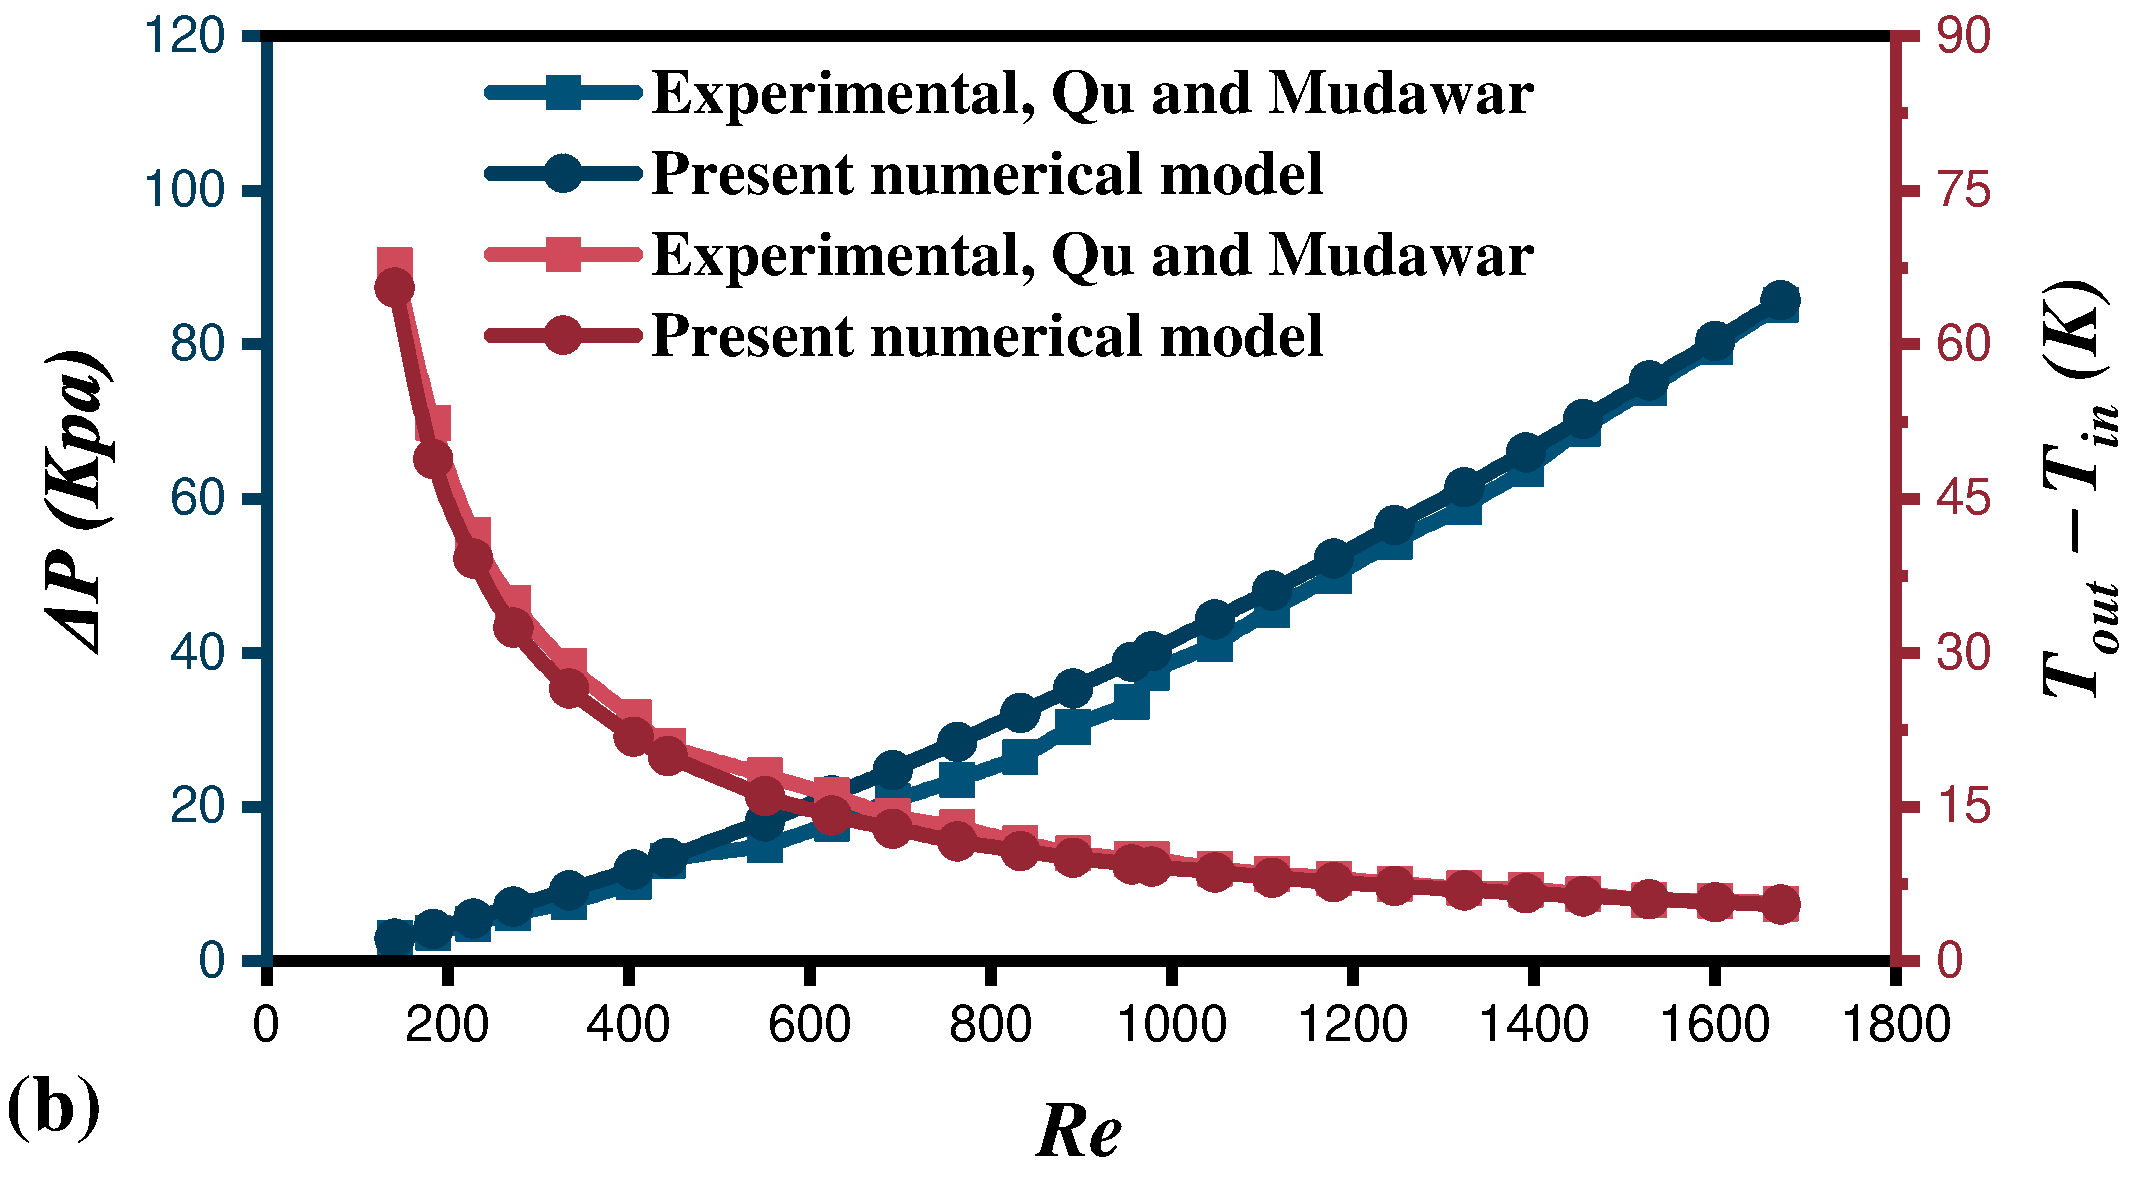
\includegraphics[width=0.4 \textwidth]{V-Qu-PT.pdf}}

    \subfloat{
        \label{fig:Yang}
        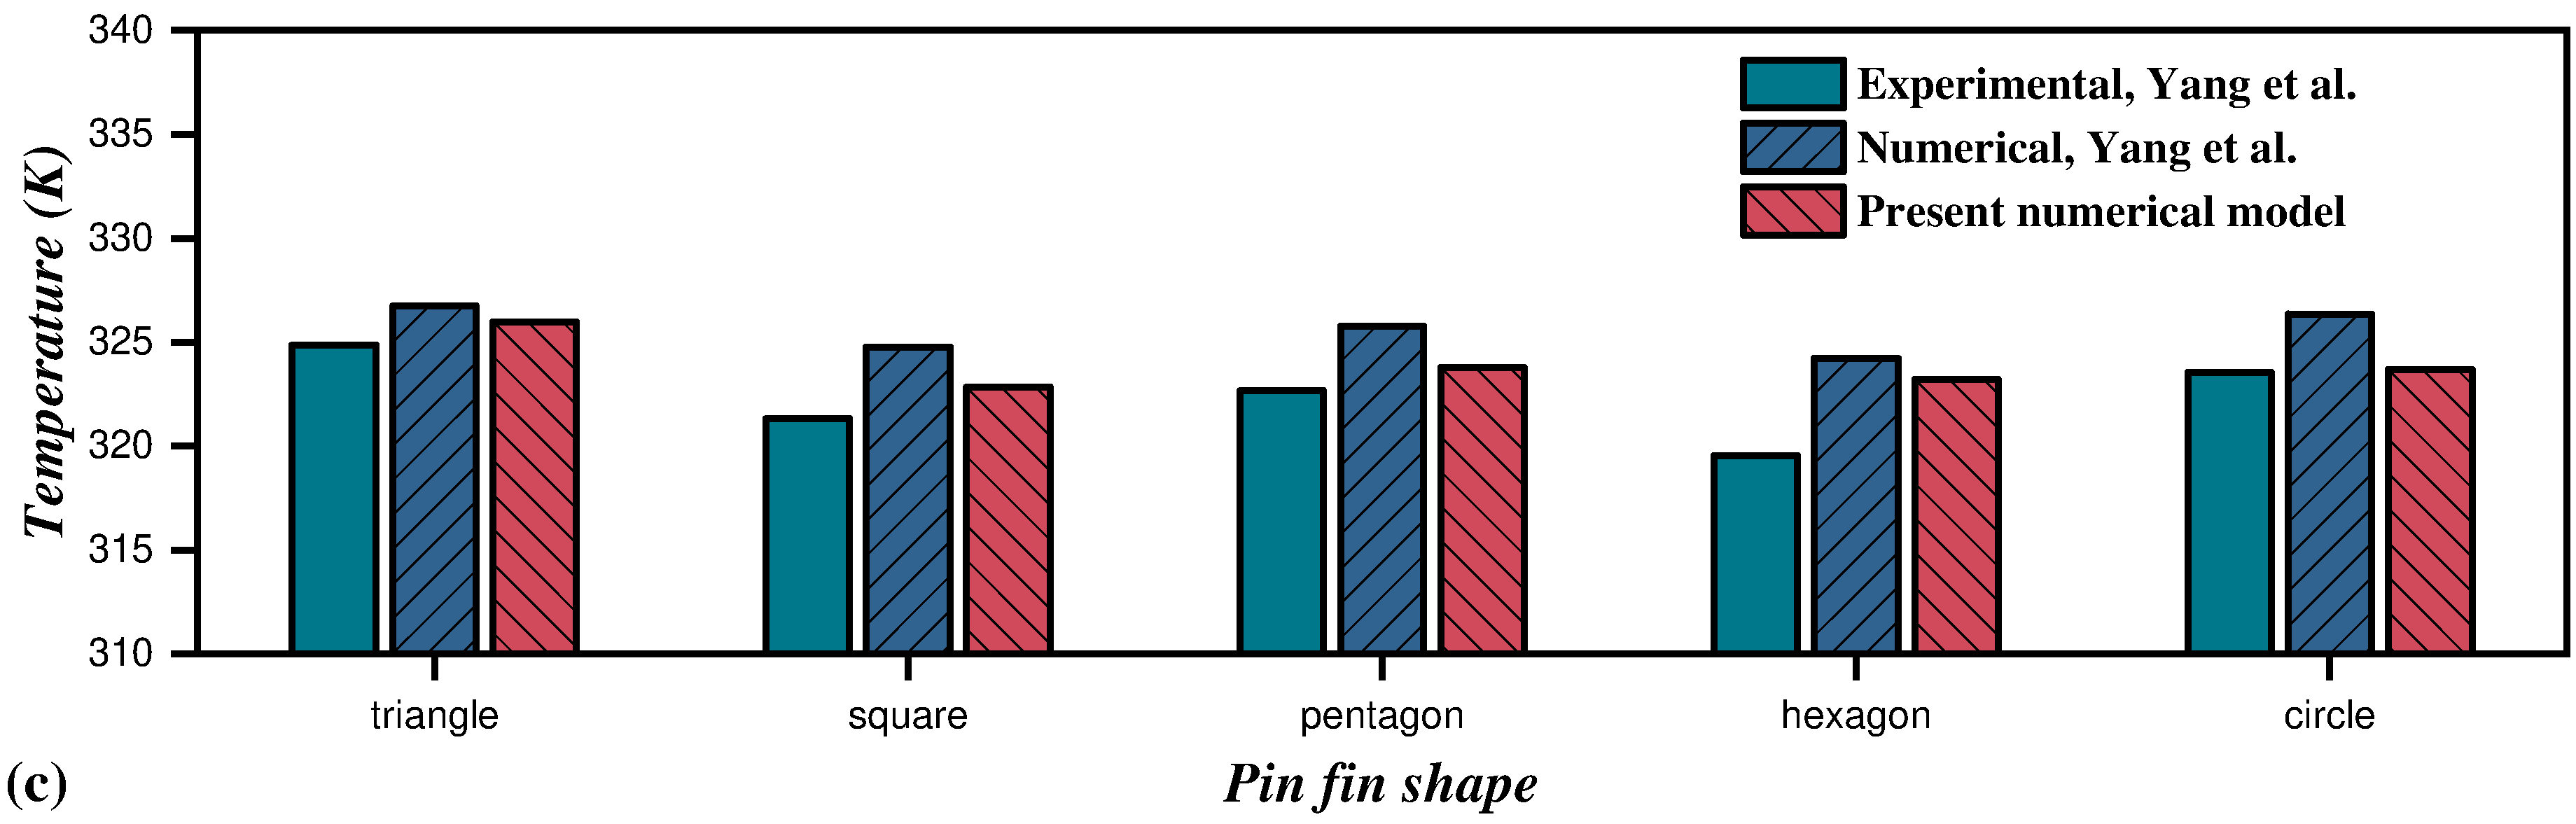
\includegraphics[width=0.75 \textwidth]{V-Yang-T.pdf}}
    \caption{Numerical validations.
        (a)Zhang et al. \cite{Zhang.Wu.ea_2022} of the microchannel heat sink at different mass flow rates for the variation of the bottom surface temperature of the microchannel heat sink.
        (b)Variation of inlet and outlet temperature difference and pressure drop in microchannels of Qu and Mudawar \cite{Qu.Mudawar_2002} at different Reynolds numbers.
        (c)Yang et al. \cite{Yang.Wang.ea_2017} of the pin-fin heat sink with the highest temperature on the bottom surface of the pin-fin heat sink for different pin-fin shapes.}
    \label{fig:Verification}
\end{figure*}

\subsection{Effect of geometric prameters on hydrothermal performance}

In order to explore the influence of the geometric




\subsubsection{The effect of relative rib height}

\subsubsection{Performance analysis}



\begin{table*}[!ht]
    \renewcommand{\arraystretch}{1.5} % 调整行距
    \centering
    \scriptsize
    \caption{Comparison with other solutions}
    \begin{threeparttable}
        \begin{tabular}{m{1.8cm}<{\raggedright}m{2.5cm}<{\raggedright}m{1.5cm}<{\raggedright}m{1.5cm}<{\raggedright}m{1cm}<{\raggedright}m{1.5cm}<{\raggedright}m{1.7cm}<{\raggedright}} \toprule
            Reference & Cooling methods & Heating area ($mm^2$) & Heat power ($W$) & Flow rate ($ml/min$) & Inlet pressure ($KPa$) & Maximum temperature ($^\circ C$) \\ \midrule
            \multirow{2}{*}{Zhang et al. \cite{Zhang.Zhang.ea_2015}} & \multirow{2}{2cm}{parallel cooling microchannels} & \multirow{2}{*}{$22\times 22$} & \multirow{2}{*}{75} & \multirow{2}{*}{58.1} & 330 & 99.52 \\ \cline{6-7}
            & & & & & $0.096^*$ & $55.7^*$ \\[5pt]
            \multirow{2}{*}{Yin et al. \cite{Yin.Li.ea_2019}} & \multirow{2}{2.2cm}{LTCC with embedded metal pillar arrays} & \multirow{2}{*}{$21\times 21$} & \multirow{2}{*}{20} & \multirow{2}{*}{18.85} & 7.12 & 74.85 \\ \cline{6-7}
            & & & & & $0.021^*$ & $57.35^*$ \\[5pt]
            \multirow{2}{*}{Liu et al. \cite{Liu.Jin.ea_2016}} & \multirow{2}{2.2cm}{LTCC with via holes and liquid metal} & \multirow{2}{*}{$10\times 10$} & \multirow{2}{*}{$30^{**}$} & \multirow{2}{*}{70} & \quad - & 83.85 \\ \cline{6-7}                                                                  
            & & & & & $0.138^*$ & $95.74^*$ \\[5pt]
            \multirow{2}{*}{Yu et al. \cite{YU.HAN.ea_2018}} & \multirow{2}{2.2cm}{LTCC with dual-layer spirals microchannels} & \multirow{2}{*}{$2\times 10$} & \multirow{2}{*}{$23^{**}$} & \multirow{2}{*}{45} & 370.7 & 84.85 \\ \cline{6-7}
            & & & & & $0.071^*$ & $55.54^*$\\\bottomrule
        \end{tabular}
        *\,\, The heat sink is MCHS-RPFEM and the coolant is deionized water.\\
        ** Heat flux($W/cm^2$)
    \end{threeparttable}
    \label{tab:Literature-comparison}
\end{table*}

